\documentclass[12pt,landscape]{article}
\usepackage{pgf, tikz}
\usetikzlibrary{arrows, automata}

\begin{document}
	\thispagestyle{empty}
	\resizebox{15cm}{10cm}{
	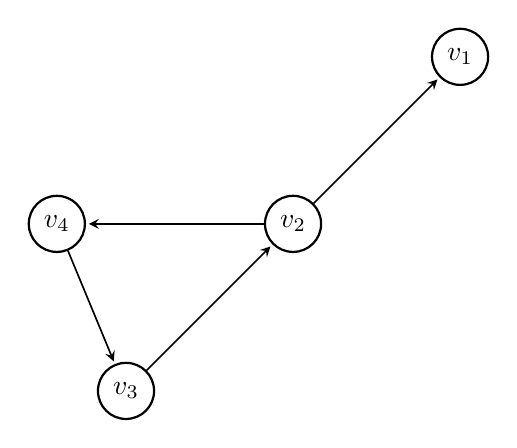
\begin{tikzpicture}[
	> = stealth, % arrow head style
	shorten > = 1pt, % don't touch arrow head to node
	auto,
	node distance = 3cm, % distance between nodes
	semithick % line style
	]
	\centering
	
	\tikzstyle{every state}=[
	draw = black,
	thick,
	fill = white,
	minimum size = 4mm
	]
	
	\node[state] (v2) {$v_2$};
	\node[state] (v1) [above right of=v2] {$v_1$};
	\node[state] (v3) [below left of=v2] {$v_3$};
	\node[state] (v4) [left of=v2] {$v_4$};
	
	\path[->] (v2) edge (v1);
	\path[->] (v3) edge (v2);
	\path[->] (v2) edge (v4);
	\path[->] (v4) edge (v3);
	
	\end{tikzpicture}
}
	
\end{document}